\section{Sample Planning Problem}

	The discussed algorithm is capable of finding paths in
	$\specialEuclideanGroup{3}$ under a wide range of situations.
	Figure~\ref{fig:stress_test_problem} shows a screenshot of a highly
	constrained planning problem designed as a stress test to strain the overall
	procedure in simulation.

	\begin{figure}[ht]
		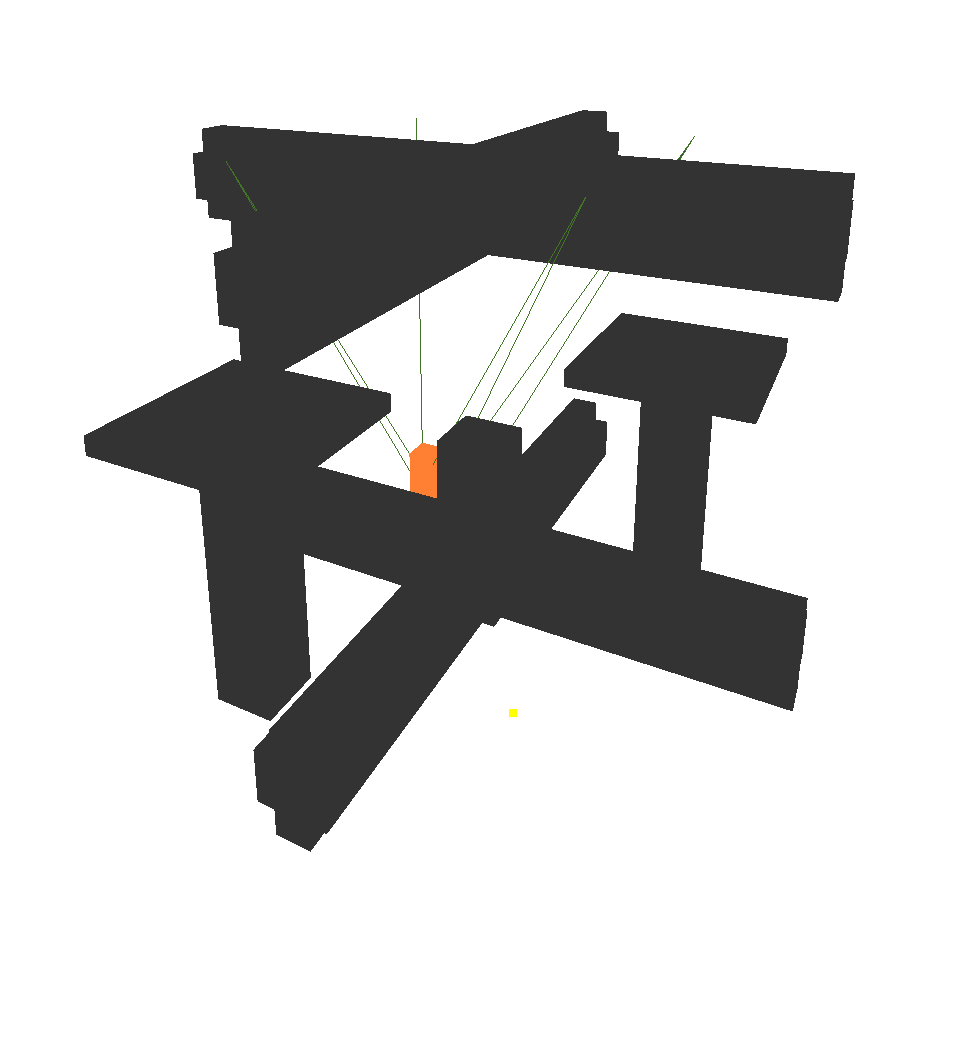
\includegraphics[width=\columnwidth]{clutter_perspective_transp}
		\caption{Sample Planning Problem}%
		\label{fig:stress_test_problem}
	\end{figure}

	As can be seen from the figure, many obstacles were placed inside the
	workspace of the \gls{cdpr}. The obstacles consist of:

	\begin{enumerate}

		\item

			A cross on the floor of the workspace. This cross is used to
			demarcate the workspace into quadrants.

		\item

			An identical cross above the workspace. This cross greatly reduces
			the mobility of the end-effector, since it can easily interfere with
			the cables.

		\item

			Two pillars with flat tops. These pillars effectively remove two
			quadrants of the workspace. The flat tops ensure that the
			end-effector can only pass in certain orientations, thereby testing
			the rotational planning of the algorithm. They also serve to provide
			regions of cable-obstacle interference when the end-effector moves
			into a quadrant.

		\item

			A small pillar in the middle of the of the workspace. This pillar
			further constrains the possible paths from one quadrant to the next.

	\end{enumerate}

	The planning algorithm was instructed to find a path to move the
	end-effector from the far quadrant in the figure to the near quadrant. Due
	to the random nature of \gls{rrt}, a slightly different path will be
	found on each iteration. One collision-free path that was found for this
	procedure is shown in
	Figure~\ref{fig:sample_trajectory_with_augmented_set_of_poses}.

	It should be noted that, since the algorithm is not optimised for such
	highly constrained cases as this problem, some iterations of the search can
	take considerable time, while others are found quite fast. As such, the
	planning step for this algorithm is more suitable for offline computation.
